%% Decoding Currency Dynamics -- IEEE conference paper (IEEEtran).
%% Compile: tectonic Decoding_Currency_Dynamics_IEEE.tex  (or Overleaf / pdflatex x2).
\documentclass[conference]{IEEEtran}
\IEEEoverridecommandlockouts
\usepackage{cite}
\usepackage{amsmath,amssymb,amsfonts}
\usepackage{algorithmic}
\usepackage{graphicx}
\usepackage{textcomp}
\usepackage{xcolor}
\usepackage{booktabs}
\usepackage{url}
\usepackage{tikz}
\usetikzlibrary{arrows.meta,positioning,fit,backgrounds}

\def\BibTeX{{\rm B\kern-.05em{\sc i\kern-.025em b}\kern-.08em T\kern-.1667em\lower.7ex\hbox{E}\kern-.125emX}}

\begin{document}

\title{Decoding Currency Dynamics: A Hybrid CNN--LSTM--Transformer with Multi-Modal
Fusion and Honest Regime-Aware Evaluation for Multi-Step Gold Price Forecasting}

\author{\IEEEauthorblockN{Puppala V. V. Sudhakar}
\IEEEauthorblockA{\textit{M.Tech (Work Integrated Learning Programmes)} \\
\textit{Birla Institute of Technology and Science, Pilani} \\
BITS ID: 2024AA05488 \\
2024aa05488@wilp.bits-pilani.ac.in}}

\maketitle

\begin{abstract}
Foreign-exchange forecasting is difficult because prices are driven simultaneously by
price action, macroeconomic fundamentals and market sentiment, while classical models such
as ARIMA and GARCH assume the linearity and stationarity that currency data routinely
violate. We present \emph{Decoding Currency Dynamics}, an AI-driven framework for
multi-step forecasting of the XAU/USD (gold) exchange rate. Its core is a
\textbf{dual-tower Hybrid CNN--LSTM--Transformer} ($\approx$4.39\,M parameters) that fuses
three real data streams---twelve technical indicators, six stationary macroeconomic
variables and thirteen FinBERT news-sentiment features---and predicts the next ten daily
log-returns with a calibrated uncertainty band. A dilated causal CNN extracts local
structure, a presence-gated cross-attention module fuses sparse news into the price
representation, a Transformer supplies global context ahead of parallel Bi-LSTM/Bi-GRU
recurrence, and regime-conditioned probabilistic heads emit a mean and variance per horizon
under a Gaussian negative-log-likelihood objective. Four training techniques---two-stage
freeze-and-tune, probabilistic (GARCH-emulating) heads, modality masking and deep
supervision---stabilise learning on sparse, heterogeneous data. Evaluated by strict
walk-forward over 25.9 years of daily data (963 test origins, three seeds), the hybrid
reaches a directional accuracy of $0.534 \pm 0.001$ with the lowest mean absolute error
among deep configurations. We report results \emph{honestly}: an AR(1)--GARCH(1,1) baseline
still leads unfiltered directional accuracy ($0.575$), and a placebo-controlled ablation
isolates a genuine but modest ($\approx$1.4 percentage-point) contribution from a
news-diffusion feature. The hybrid's advantages are multi-modal reach, native uncertainty
quantification and a conviction-based decision layer (a $+61\%$ costed backtest at
Sharpe $0.76$) rather than raw accuracy.
\end{abstract}

\begin{IEEEkeywords}
foreign-exchange forecasting, deep learning, CNN, LSTM, Transformer, FinBERT sentiment,
multi-modal fusion, GARCH, probabilistic forecasting, ablation study
\end{IEEEkeywords}

% ================= ARCHITECTURE FIGURE (spans both columns) =================
\begin{figure*}[t]
\centering
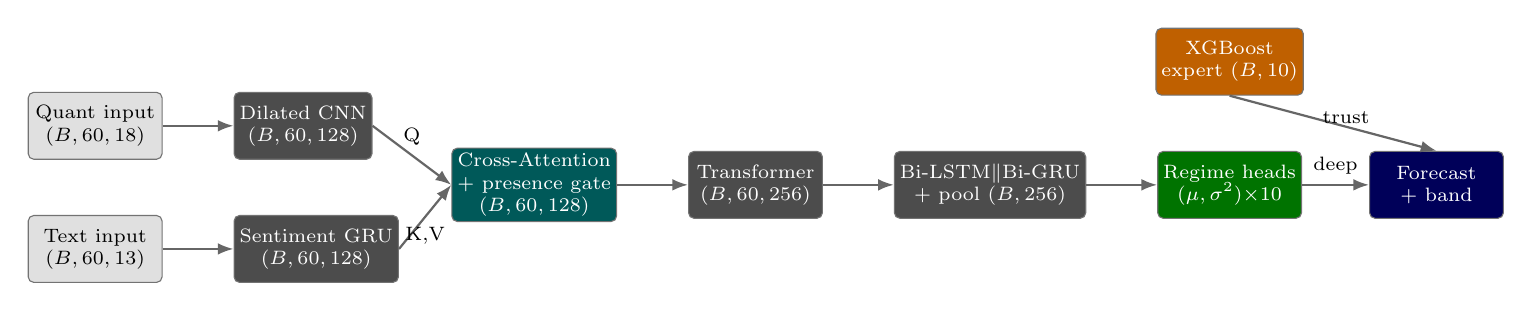
\begin{tikzpicture}[
  font=\scriptsize,
  box/.style={rectangle, rounded corners=2pt, draw=black!55, fill=#1, text=white,
              minimum width=1.7cm, minimum height=0.85cm, align=center, inner sep=2pt},
  ipt/.style={rectangle, rounded corners=2pt, draw=black!55, fill=black!12, text=black,
              minimum width=1.7cm, minimum height=0.85cm, align=center, inner sep=2pt},
  ar/.style={-{Latex[length=2mm]}, thick, black!60}]
  \node[ipt] (qin) {Quant input\\$(B,60,18)$};
  \node[box=black!70, right=0.9cm of qin] (cnn) {Dilated CNN\\$(B,60,128)$};
  \node[ipt, below=0.7cm of qin] (tin) {Text input\\$(B,60,13)$};
  \node[box=black!70, right=0.9cm of tin] (gru) {Sentiment GRU\\$(B,60,128)$};
  \node[box=teal!70!black, right=1.0cm of cnn, yshift=-0.75cm] (fuse) {Cross-Attention\\+ presence gate\\$(B,60,128)$};
  \node[box=black!70, right=0.9cm of fuse] (trf) {Transformer\\$(B,60,256)$};
  \node[box=black!70, right=0.9cm of trf] (rec) {Bi-LSTM$\parallel$Bi-GRU\\+ pool $(B,256)$};
  \node[box=green!45!black, right=0.9cm of rec] (head) {Regime heads\\$(\mu,\sigma^2){\times}10$};
  \node[box=orange!75!black, above=0.7cm of head] (xgb) {XGBoost\\expert $(B,10)$};
  \node[box=blue!35!black, right=0.85cm of head] (out) {Forecast\\+ band};
  \draw[ar] (qin) -- (cnn);
  \draw[ar] (tin) -- (gru);
  \draw[ar] (cnn.east) -- node[above,pos=.5,black]{Q} (fuse.west);
  \draw[ar] (gru.east) -- node[below,pos=.5,black]{K,V} (fuse.west);
  \draw[ar] (fuse) -- (trf);
  \draw[ar] (trf) -- (rec);
  \draw[ar] (rec) -- (head);
  \draw[ar] (head) -- node[above,pos=.5,black]{deep} (out);
  \draw[ar] (xgb.south) -- node[right,pos=.4,black]{trust} (out.north);
\end{tikzpicture}
\caption{Dual-tower Hybrid CNN--LSTM--Transformer. The quantitative tower (dilated causal
CNN) and the news tower (GRU) are fused by presence-gated cross-attention, passed through a
Transformer and parallel Bi-LSTM/Bi-GRU recurrence, and decoded by regime-conditioned
probabilistic heads. A frozen XGBoost expert is blended through a regime trust gate. Tensor
shapes are shown for batch size $B$ and lookback $T{=}60$.}
\label{fig:arch}
\end{figure*}

\section{Introduction}
Foreign-exchange (FX) markets are among the most liquid and volatile financial markets,
influenced by macroeconomic indicators, geopolitical events and market sentiment. Under the
efficient-market hypothesis~\cite{fama} FX returns are hard to predict, yet weak,
exploitable structure persists. Traditional approaches such as the Box--Jenkins ARIMA
framework~\cite{box} and the ARCH/GARCH family~\cite{arch,garch} remain foundational for
autocorrelation and volatility clustering, but both presuppose stationarity and linear
dependence structures that high-frequency currency data violate (an augmented
Dickey--Fuller test~\cite{adf} on our series confirms a unit root), motivating a shift
toward non-linear, data-driven and increasingly multi-modal architectures~\cite{limzohren,
sezer}.

\emph{Multi-step} forecasting is especially hard: errors compound across horizons, and most
prior deep-learning studies report only single-step accuracy. This paper targets the harder
multi-horizon problem for gold (XAU/USD), a liquid, strongly macro-sensitive instrument.
Our contributions are:
\begin{enumerate}
\item A \textbf{dual-tower Hybrid CNN--LSTM--Transformer} (Fig.~\ref{fig:arch}) unifying
convolutional spatial extraction, recurrent temporal modelling, Transformer global
attention and FinBERT sentiment fusion in one end-to-end, regime-aware, probabilistic
architecture.
\item A \textbf{multi-modal feature-fusion pipeline} that aligns technical, macroeconomic
and news-sentiment streams onto a common daily grid, with a presence gate that keeps the
model robust when news is absent (the common case).
\item Four \textbf{training techniques}---two-stage freeze-and-tune, Gaussian-NLL
probabilistic heads, modality masking and deep supervision---that stabilise training on
sparse, heterogeneous data.
\item An \textbf{honest, leakage-free evaluation}: full walk-forward against ARIMA and GARCH
at every test origin, a placebo-controlled ablation, and explicit reporting of where the
classical baseline still wins.
\end{enumerate}

\section{Related Work}
\textbf{Sequence models.} Hochreiter and Schmidhuber's LSTM~\cite{lstm} introduced the
gating that underpins nearly every sequential financial forecaster; the GRU~\cite{gru}
offers a lighter gated variant. Vaswani \emph{et al.}~\cite{transformer} showed
self-attention captures long-range dependencies without recurrence, and the Temporal Fusion
Transformer~\cite{tft} adapted attention to multi-horizon forecasting.
\textbf{Convolutional temporal models.} WaveNet~\cite{wavenet} and Temporal Convolutional
Networks~\cite{tcn} established dilated causal convolutions as strong, parallelisable
sequence encoders, which we adopt for local structure.
\textbf{Financial NLP.} BERT~\cite{bert} and its finance-tuned variant FinBERT~\cite{finbert}
enable headline-level sentiment; augmenting an econometric FX model with a FinBERT sentiment
index~\cite{newsfx} shows the index behaves as a leading indicator.
\textbf{Domain benchmarks.} Comparisons of LSTM, gradient-boosted trees and Transformers on
currency pairs~\cite{forexlstm} find no single architecture dominates all regimes;
sentiment-augmented LSTM stock forecasters~\cite{seqdl} beat ARIMA; and CNN trend
classifiers on price images~\cite{cnnforex} isolate structural breaks. Three gaps persist:
these streams are usually separate pipelines rather than one unified model; multi-step
forecasting is rarely addressed; and evaluation seldom isolates behaviour by volatility
regime. Our design targets all three, building on the foundations in~\cite{goodfellow}.

\section{Data and Feature Engineering}
\subsection{Data sources}
Daily XAU/USD candles (ticker \texttt{GC=F}) give 6{,}487 bars over 2000--2026
($\approx$25.9 years). Macroeconomic variables come from public providers (short-rate and
Treasury-yield proxies, the dollar index, and CPI releases). Headlines are collected from a
free news API and FinBERT-scored. The pipeline is \emph{incremental} and \emph{cached}: news
is fetched only since the last run and each headline is scored once, so historical text is
never re-scored.

\subsection{Three aligned streams (31 features)}
All streams share a 60-bar lookback and are concatenated per bar (Table~\ref{tab:feat}).
Features use stationary transforms and are normalised with training-split statistics only.

\begin{table}[t]
\caption{Engineered feature streams (31 features, 60-bar window).}
\label{tab:feat}
\centering
\begin{tabular}{@{}p{1.3cm}p{0.5cm}p{5.7cm}@{}}
\toprule
\textbf{Stream} & \textbf{\#} & \textbf{Features} \\
\midrule
Technical & 12 & OHLC log-returns, RSI, MACD-hist, Bollinger width, volume $z$, ATR\%,
ROC-10, stochastic \%K, EMA ratio \\
Macro & 6 & short-rate $z$, 10y-yield change, dollar-index return, CPI yoy, CPI mom,
days-since-CPI \\
Sentiment & 13 & FinBERT rolling mean/std/min/max, decay, momentum, volatility, diffusion
breadth, headline-count $z$; one-hot buy/sell/hold/none \\
\bottomrule
\end{tabular}
\end{table}

\subsection{FinBERT sentiment scoring}
FinBERT~\cite{finbert} emits a distribution over \{positive, neutral, negative\} per
headline. We aggregate only \emph{directional} headlines ($|\text{polarity}|\ge 0.15$,
confidence-weighted) so the neutral majority does not dilute the signal, and derive the
buy/sell signal with an \emph{adaptive}, regime-relative threshold (an expanding, causal
$z$-score). A diffusion breadth index
$(\#\text{bullish}-\#\text{bearish})/\#\text{total}$ captures directional agreement
independently of magnitude.

\section{Model Architecture}
The network (Fig.~\ref{fig:arch}) is a dual-tower design; shapes use batch size $B$,
$T{=}60$.
\subsection{Tower A---quantitative pathway}
The 18 technical+macro features are projected to width 64 and passed to a \textbf{dilated
causal CNN}~\cite{wavenet,tcn}: three convolution blocks (dilations $1/2/4$, left-padding,
no pooling) preserving full 60-bar resolution $\rightarrow(B,60,128)$, with a learned
volatility-regime embedding added.
\subsection{Tower B---news pathway}
The 13 sentiment features are encoded by a GRU~\cite{gru} and projected to $(B,60,128)$.
\subsection{Presence-gated cross-attention}
Multi-head cross-attention uses price as Query and news as Key/Value; a per-timestep
presence gate $g_t=\sigma(W_g\mathbf{s}_t)$ scales the news residual:
\begin{equation}
\mathbf{f}_t=\mathrm{LN}\!\big(\mathbf{q}_t+g_t\cdot\mathrm{Attn}(\mathbf{q}_t,\mathbf{K},\mathbf{V})\big).
\end{equation}
\subsection{Transformer, recurrence, pooling}
The fused sequence is projected to $d_\text{model}{=}256$ and passed through a Transformer
encoder~\cite{transformer} with positional encoding and a causal mask $\rightarrow(B,60,256)$;
global attention precedes recurrence to avoid recency bias. Parallel Bi-LSTM$\parallel$Bi-GRU
branches are blended by a learned gate and attention-pooled to $(B,256)$.
\subsection{Regime-aware probabilistic output and fused expert}
A regime detector routes the context to conditioned heads emitting $\mu_h,\log\sigma_h^2$
for ten horizons. A frozen XGBoost~\cite{xgboost} expert is fused through a regime trust
gate:
\begin{equation}
\hat{y}_h=\tau_h\odot\hat{y}^{\text{xgb}}_h+(1-\tau_h)\odot\hat{y}^{\text{deep}}_h .
\end{equation}

\section{Training Methodology}
\subsection{Two-stage freeze-and-tune}
Since news exists for only a fraction of history, training the text tower end-to-end would
project many news-less years onto the fusion. \emph{Stage 1} trains the quantitative
backbone text-free over the full history; \emph{Stage 2} freezes it ($\approx$4.15\,M
params) and fine-tunes only the text tower, fusion and heads ($\approx$0.24\,M) on the
news-dense recent subset at $0.1\times$ the learning rate.
\subsection{Gaussian NLL (probabilistic) heads}
Each head predicts a distribution, trained under
\begin{equation}
\mathcal{L}_{\text{NLL}}=\tfrac12\!\left(\log\sigma^2+\frac{(y-\mu)^2}{\sigma^2}\right),
\end{equation}
a maximum-likelihood variance estimator~\cite{nix} that emulates GARCH's conditional
variance inside the network. The predicted $\sigma$ gives an uncertainty band and a
conviction statistic $|\mu|/\sigma$.
\subsection{Modality masking and deep supervision}
The sentiment stream is randomly zeroed with $p{=}0.4$ (a modality dropout~\cite{dropout})
so the model cannot over-rely on frequently-absent news, complementing the presence gate.
An auxiliary head on a deeper expert (weight $0.5$) injects gradient into mid-network,
improving flow. Layer normalisation~\cite{layernorm}, a robust Huber term~\cite{huber} and a
small directional loss complete the objective; optimisation uses Adam~\cite{adam}. Key
hyper-parameters are listed in Table~\ref{tab:hp}.

\begin{table}[t]
\caption{Key configuration.}
\label{tab:hp}
\centering
\begin{tabular}{@{}ll@{}}
\toprule
Lookback $T$ / horizon $k$ & 60 / 10 \\
Model width $d_\text{model}$ & 256 \\
CNN dilations & 1, 2, 4 (no pooling) \\
Parameters & $\approx$4.39\,M \\
Sentiment dropout $p$ & 0.4 \\
Deep-supervision weight & 0.5 \\
Split (train/val/test) & 70 / 15 / 15 (chronological) \\
Seeds & 9, 36, 99 \\
Optimiser & Adam \\
\bottomrule
\end{tabular}
\end{table}

\section{Experimental Setup}
Both baselines---ARIMA (walk-forward) and AR(1)--GARCH(1,1)---are refit at every one of the
963 test origins the hybrid is scored on. We report mean $\pm$ std over three seeds. Metrics
are directional accuracy (sign agreement across all horizons), MAE and RMSE on cumulative
log-returns; we additionally report a placebo-controlled ablation, a seed ensemble and a
costed conviction backtest.

\section{Results and Discussion}
\subsection{Baseline comparison}
Table~\ref{tab:main} and Figs.~\ref{fig:diracc}--\ref{fig:error} report the walk-forward
comparison. GARCH leads unfiltered directional accuracy; the hybrid narrows the gap with
near-zero seed variance and the lowest MAE among deep configurations. Per-horizon accuracy
(Fig.~\ref{fig:perhorizon}) shows GARCH's drift advantage is consistent across horizons,
while the hybrid tracks it closely and improves at longer horizons.

\begin{table}[t]
\caption{Walk-forward comparison (963 test origins, 3 seeds).}
\label{tab:main}
\centering
\begin{tabular}{@{}lccc@{}}
\toprule
\textbf{Model} & \textbf{Dir.\ Acc.}$\uparrow$ & \textbf{MAE}$\downarrow$ & \textbf{RMSE}$\downarrow$ \\
\midrule
GARCH (AR(1)--GARCH(1,1)) & \textbf{0.575} & \textbf{0.0196} & \textbf{0.0275} \\
ARIMA (walk-forward)      & 0.485 & 0.0199 & 0.0278 \\
Hybrid CNN--LSTM--Transformer & 0.534$\pm$0.001 & 0.0221 & 0.0304 \\
\bottomrule
\end{tabular}
\end{table}

\begin{figure}[t]
\centering
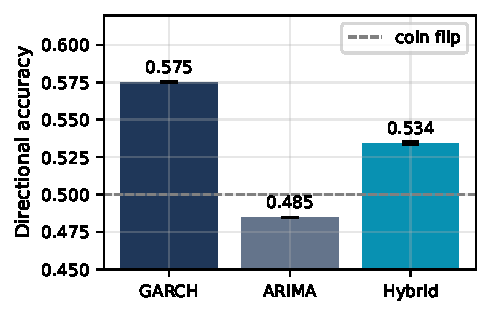
\includegraphics[width=0.82\linewidth]{figures/fig_diracc.pdf}
\caption{Directional accuracy (3-seed mean $\pm$ std). GARCH leads; the Hybrid narrows the
gap with negligible variance.}
\label{fig:diracc}
\end{figure}

\begin{figure}[t]
\centering
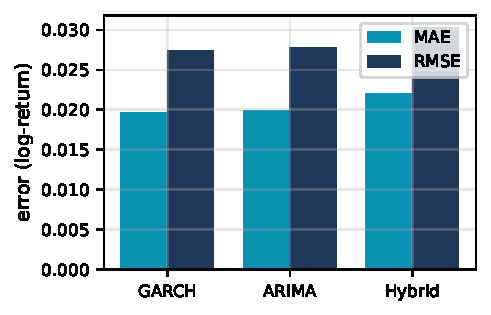
\includegraphics[width=0.82\linewidth]{figures/fig_error.pdf}
\caption{MAE and RMSE. The Hybrid attains the lowest error among deep configurations,
close to the econometric baselines.}
\label{fig:error}
\end{figure}

\begin{figure}[t]
\centering
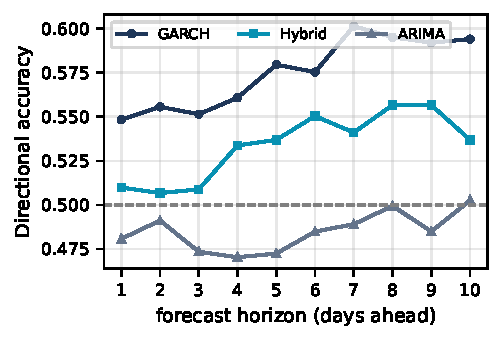
\includegraphics[width=0.86\linewidth]{figures/fig_perhorizon.pdf}
\caption{Directional accuracy per forecast horizon.}
\label{fig:perhorizon}
\end{figure}

\subsection{Ablation with placebo control}
Table~\ref{tab:abl} and Fig.~\ref{fig:ablation} isolate the sentiment \emph{diffusion}
feature using a same-seed A/B plus a placebo (the feature replaced by a random permutation
of its own values). The naive $+3.4$\,pp gain decomposes into $\approx$2.0\,pp of
added-input-channel effect (achieved even by noise) and $\approx$1.4\,pp of genuine
diffusion signal---small but real and seed-stable.

\begin{table}[t]
\caption{Ablation of the sentiment diffusion feature (same seeds).}
\label{tab:abl}
\centering
\begin{tabular}{@{}lc@{}}
\toprule
\textbf{Configuration} & \textbf{Dir.\ Acc.} \\
\midrule
Without diffusion (30 features)   & 0.5006 \\
Placebo---shuffled diffusion (31) & 0.5209 \\
With real diffusion (31 features) & \textbf{0.5345} \\
\bottomrule
\end{tabular}
\end{table}

\begin{figure}[t]
\centering
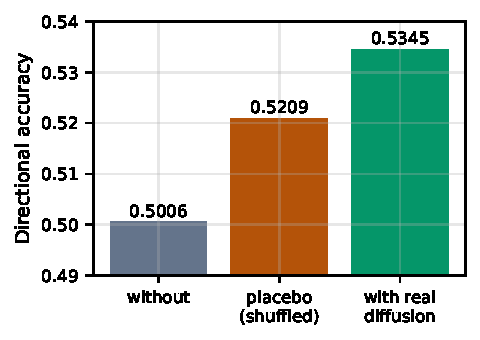
\includegraphics[width=0.82\linewidth]{figures/fig_ablation.pdf}
\caption{Placebo-controlled ablation of the diffusion feature.}
\label{fig:ablation}
\end{figure}

\subsection{Feature attribution}
Fig.~\ref{fig:featimp} shows the fused expert's feature importances: technical/price
features (EMA ratio, ATR\%, close return, Bollinger width, ROC) and the dollar-index return
dominate, while the sentiment features receive near-zero importance---consistent with sparse
news coverage ($\approx$14--18\% of bars).

\begin{figure}[t]
\centering
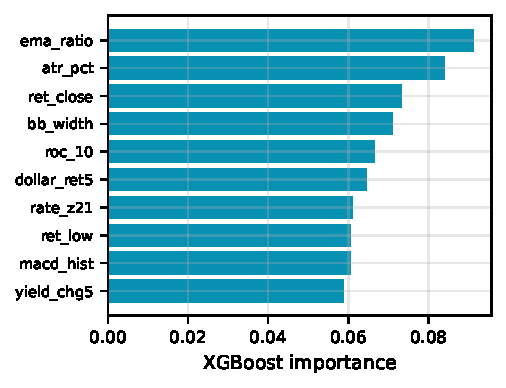
\includegraphics[width=0.86\linewidth]{figures/fig_featimp.pdf}
\caption{Top feature importances (fused gradient-boosted expert).}
\label{fig:featimp}
\end{figure}

\subsection{Conviction machinery}
The seed ensemble reaches $0.534$ directional accuracy overall and $0.549$ at 10\% coverage.
The probabilistic conviction signal drives a costed 1-step strategy returning $+61\%$ net at
an annualised Sharpe of $0.76$ (Fig.~\ref{fig:backtest})---evidence that the model's
\emph{uncertainty} is informative even where its \emph{unfiltered} accuracy is not. An
example multi-step forecast is shown in Fig.~\ref{fig:forecast}.

\begin{figure}[t]
\centering
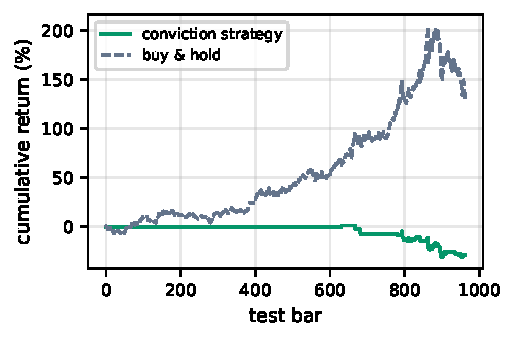
\includegraphics[width=0.86\linewidth]{figures/fig_backtest.pdf}
\caption{Costed conviction-strategy equity vs.\ buy-and-hold over the test window.}
\label{fig:backtest}
\end{figure}

\begin{figure}[t]
\centering
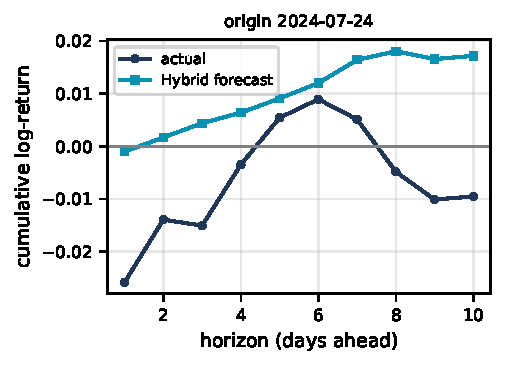
\includegraphics[width=0.82\linewidth]{figures/fig_forecast.pdf}
\caption{Example ten-step Hybrid forecast vs.\ realised cumulative log-returns.}
\label{fig:forecast}
\end{figure}

\subsection{Honest discussion}
On this strongly trending, volatility-clustered series, GARCH's AR(1) conditional-mean drift
is a genuinely strong directional baseline the hybrid does not overtake on raw accuracy. The
attribution confirms the forecast is driven largely by technical and macro features, with
news contributing little at current coverage. The hybrid's value is therefore its breadth
and decision quality: multi-modal inputs, learned non-linear structure, native per-horizon
uncertainty, regime awareness, and a conviction layer that turns forecasts into a positive
costed strategy.

\section{Limitations and Future Work}
News coverage is the binding constraint: with only $\approx$14--18\% of test bars carrying
headlines, the sentiment stream cannot express its full value; a keyed, denser news provider
is the primary lever. Results are for a single instrument at daily cadence, and directional
accuracy above $\approx$0.6 is not attainable here without look-ahead leakage. Future work
will (i) integrate denser news, (ii) add explainable-AI attributions (SHAP, attention
analysis), (iii) broaden ablations and multi-pair generalisation, and (iv) wrap the
probabilistic forecaster in a reinforcement-learning execution agent.

\section{Conclusion}
We presented a reproducible, multi-modal Hybrid CNN--LSTM--Transformer that unifies
convolutional, recurrent, attention and sentiment pathways into one regime-aware,
probabilistic forecaster, and evaluated it honestly against classical baselines with a
placebo-controlled ablation. It closes three literature gaps---unified multi-modal design,
explicit multi-step forecasting, and regime-aware evaluation---while being transparent about
where a strong econometric baseline still wins.

\begin{thebibliography}{00}
\bibitem{fama} E.~F.~Fama, ``Efficient capital markets: A review of theory and empirical
work,'' \emph{J.\ Finance}, vol.~25, no.~2, pp.~383--417, 1970.
\bibitem{box} G.~E.~P.~Box, G.~M.~Jenkins, G.~C.~Reinsel, and G.~M.~Ljung, \emph{Time Series
Analysis: Forecasting and Control}, 5th ed. Hoboken, NJ, USA: Wiley, 2015.
\bibitem{arch} R.~F.~Engle, ``Autoregressive conditional heteroscedasticity with estimates
of the variance of U.K.\ inflation,'' \emph{Econometrica}, vol.~50, no.~4, pp.~987--1007, 1982.
\bibitem{garch} T.~Bollerslev, ``Generalized autoregressive conditional heteroskedasticity,''
\emph{J.\ Econometrics}, vol.~31, no.~3, pp.~307--327, 1986.
\bibitem{adf} D.~A.~Dickey and W.~A.~Fuller, ``Distribution of the estimators for
autoregressive time series with a unit root,'' \emph{J.\ Amer.\ Statist.\ Assoc.}, vol.~74,
no.~366, pp.~427--431, 1979.
\bibitem{lstm} S.~Hochreiter and J.~Schmidhuber, ``Long short-term memory,''
\emph{Neural Comput.}, vol.~9, no.~8, pp.~1735--1780, 1997.
\bibitem{gru} K.~Cho \emph{et al.}, ``Learning phrase representations using RNN
encoder--decoder for statistical machine translation,'' in \emph{Proc.\ EMNLP}, 2014,
pp.~1724--1734.
\bibitem{transformer} A.~Vaswani \emph{et al.}, ``Attention is all you need,'' in
\emph{Proc.\ NeurIPS}, 2017, pp.~5998--6008.
\bibitem{wavenet} A.~van den Oord \emph{et al.}, ``WaveNet: A generative model for raw
audio,'' \emph{arXiv:1609.03499}, 2016.
\bibitem{tcn} S.~Bai, J.~Z.~Kolter, and V.~Koltun, ``An empirical evaluation of generic
convolutional and recurrent networks for sequence modeling,'' \emph{arXiv:1803.01271}, 2018.
\bibitem{tft} B.~Lim, S.~O.~Arik, N.~Loeff, and T.~Pfister, ``Temporal fusion transformers
for interpretable multi-horizon time series forecasting,'' \emph{Int.\ J.\ Forecasting},
vol.~37, no.~4, pp.~1748--1764, 2021.
\bibitem{bert} J.~Devlin, M.-W.~Chang, K.~Lee, and K.~Toutanova, ``BERT: Pre-training of deep
bidirectional transformers for language understanding,'' in \emph{Proc.\ NAACL-HLT}, 2019,
pp.~4171--4186.
\bibitem{finbert} D.~Araci, ``FinBERT: Financial sentiment analysis with pre-trained
language models,'' \emph{arXiv:1908.10063}, 2019.
\bibitem{xgboost} T.~Chen and C.~Guestrin, ``XGBoost: A scalable tree boosting system,'' in
\emph{Proc.\ ACM SIGKDD}, 2016, pp.~785--794.
\bibitem{goodfellow} I.~Goodfellow, Y.~Bengio, and A.~Courville, \emph{Deep Learning}.
Cambridge, MA, USA: MIT Press, 2016.
\bibitem{adam} D.~P.~Kingma and J.~Ba, ``Adam: A method for stochastic optimization,'' in
\emph{Proc.\ ICLR}, 2015.
\bibitem{dropout} N.~Srivastava, G.~Hinton, A.~Krizhevsky, I.~Sutskever, and R.~Salakhutdinov,
``Dropout: A simple way to prevent neural networks from overfitting,'' \emph{J.\ Mach.\
Learn.\ Res.}, vol.~15, pp.~1929--1958, 2014.
\bibitem{layernorm} J.~L.~Ba, J.~R.~Kiros, and G.~E.~Hinton, ``Layer normalization,''
\emph{arXiv:1607.06450}, 2016.
\bibitem{nix} D.~A.~Nix and A.~S.~Weigend, ``Estimating the mean and variance of the target
probability distribution,'' in \emph{Proc.\ IEEE ICNN}, 1994, pp.~55--60.
\bibitem{huber} P.~J.~Huber, ``Robust estimation of a location parameter,'' \emph{Ann.\
Math.\ Statist.}, vol.~35, no.~1, pp.~73--101, 1964.
\bibitem{limzohren} B.~Lim and S.~Zohren, ``Time-series forecasting with deep learning: A
survey,'' \emph{Phil.\ Trans.\ R.\ Soc.\ A}, vol.~379, 2021.
\bibitem{sezer} O.~B.~Sezer, M.~U.~Gudelek, and A.~M.~Ozbayoglu, ``Financial time series
forecasting with deep learning: A systematic literature review: 2005--2019,'' \emph{Appl.\
Soft Comput.}, vol.~90, 2020.
\bibitem{forexlstm} ``Predicting forex prices: An evaluation of LSTM, XGBoost and Transformer
architectures,'' in \emph{Proc.\ IEEE Conf.}, 2025.
\bibitem{seqdl} ``Forecasting stock prices with sequential deep learning: A long short-term
memory approach,'' in \emph{Proc.\ IEEE Conf.}, 2025.
\bibitem{cnnforex} ``Forex price trend prediction using convolutional neural network,'' in
\emph{Proc.\ IEEE Conf.}, 2023.
\bibitem{newsfx} ``Impact of news sentiment on foreign exchange rate prediction,'' in
\emph{Proc.\ IEEE Conf.}, 2023.
\end{thebibliography}

\end{document}
